% ===== STEP 2: Define Search Strategy =====
% This section covers:
% - Search strategy development
% - Documentation of search process

\begin{figure*}[th]
	\centering
	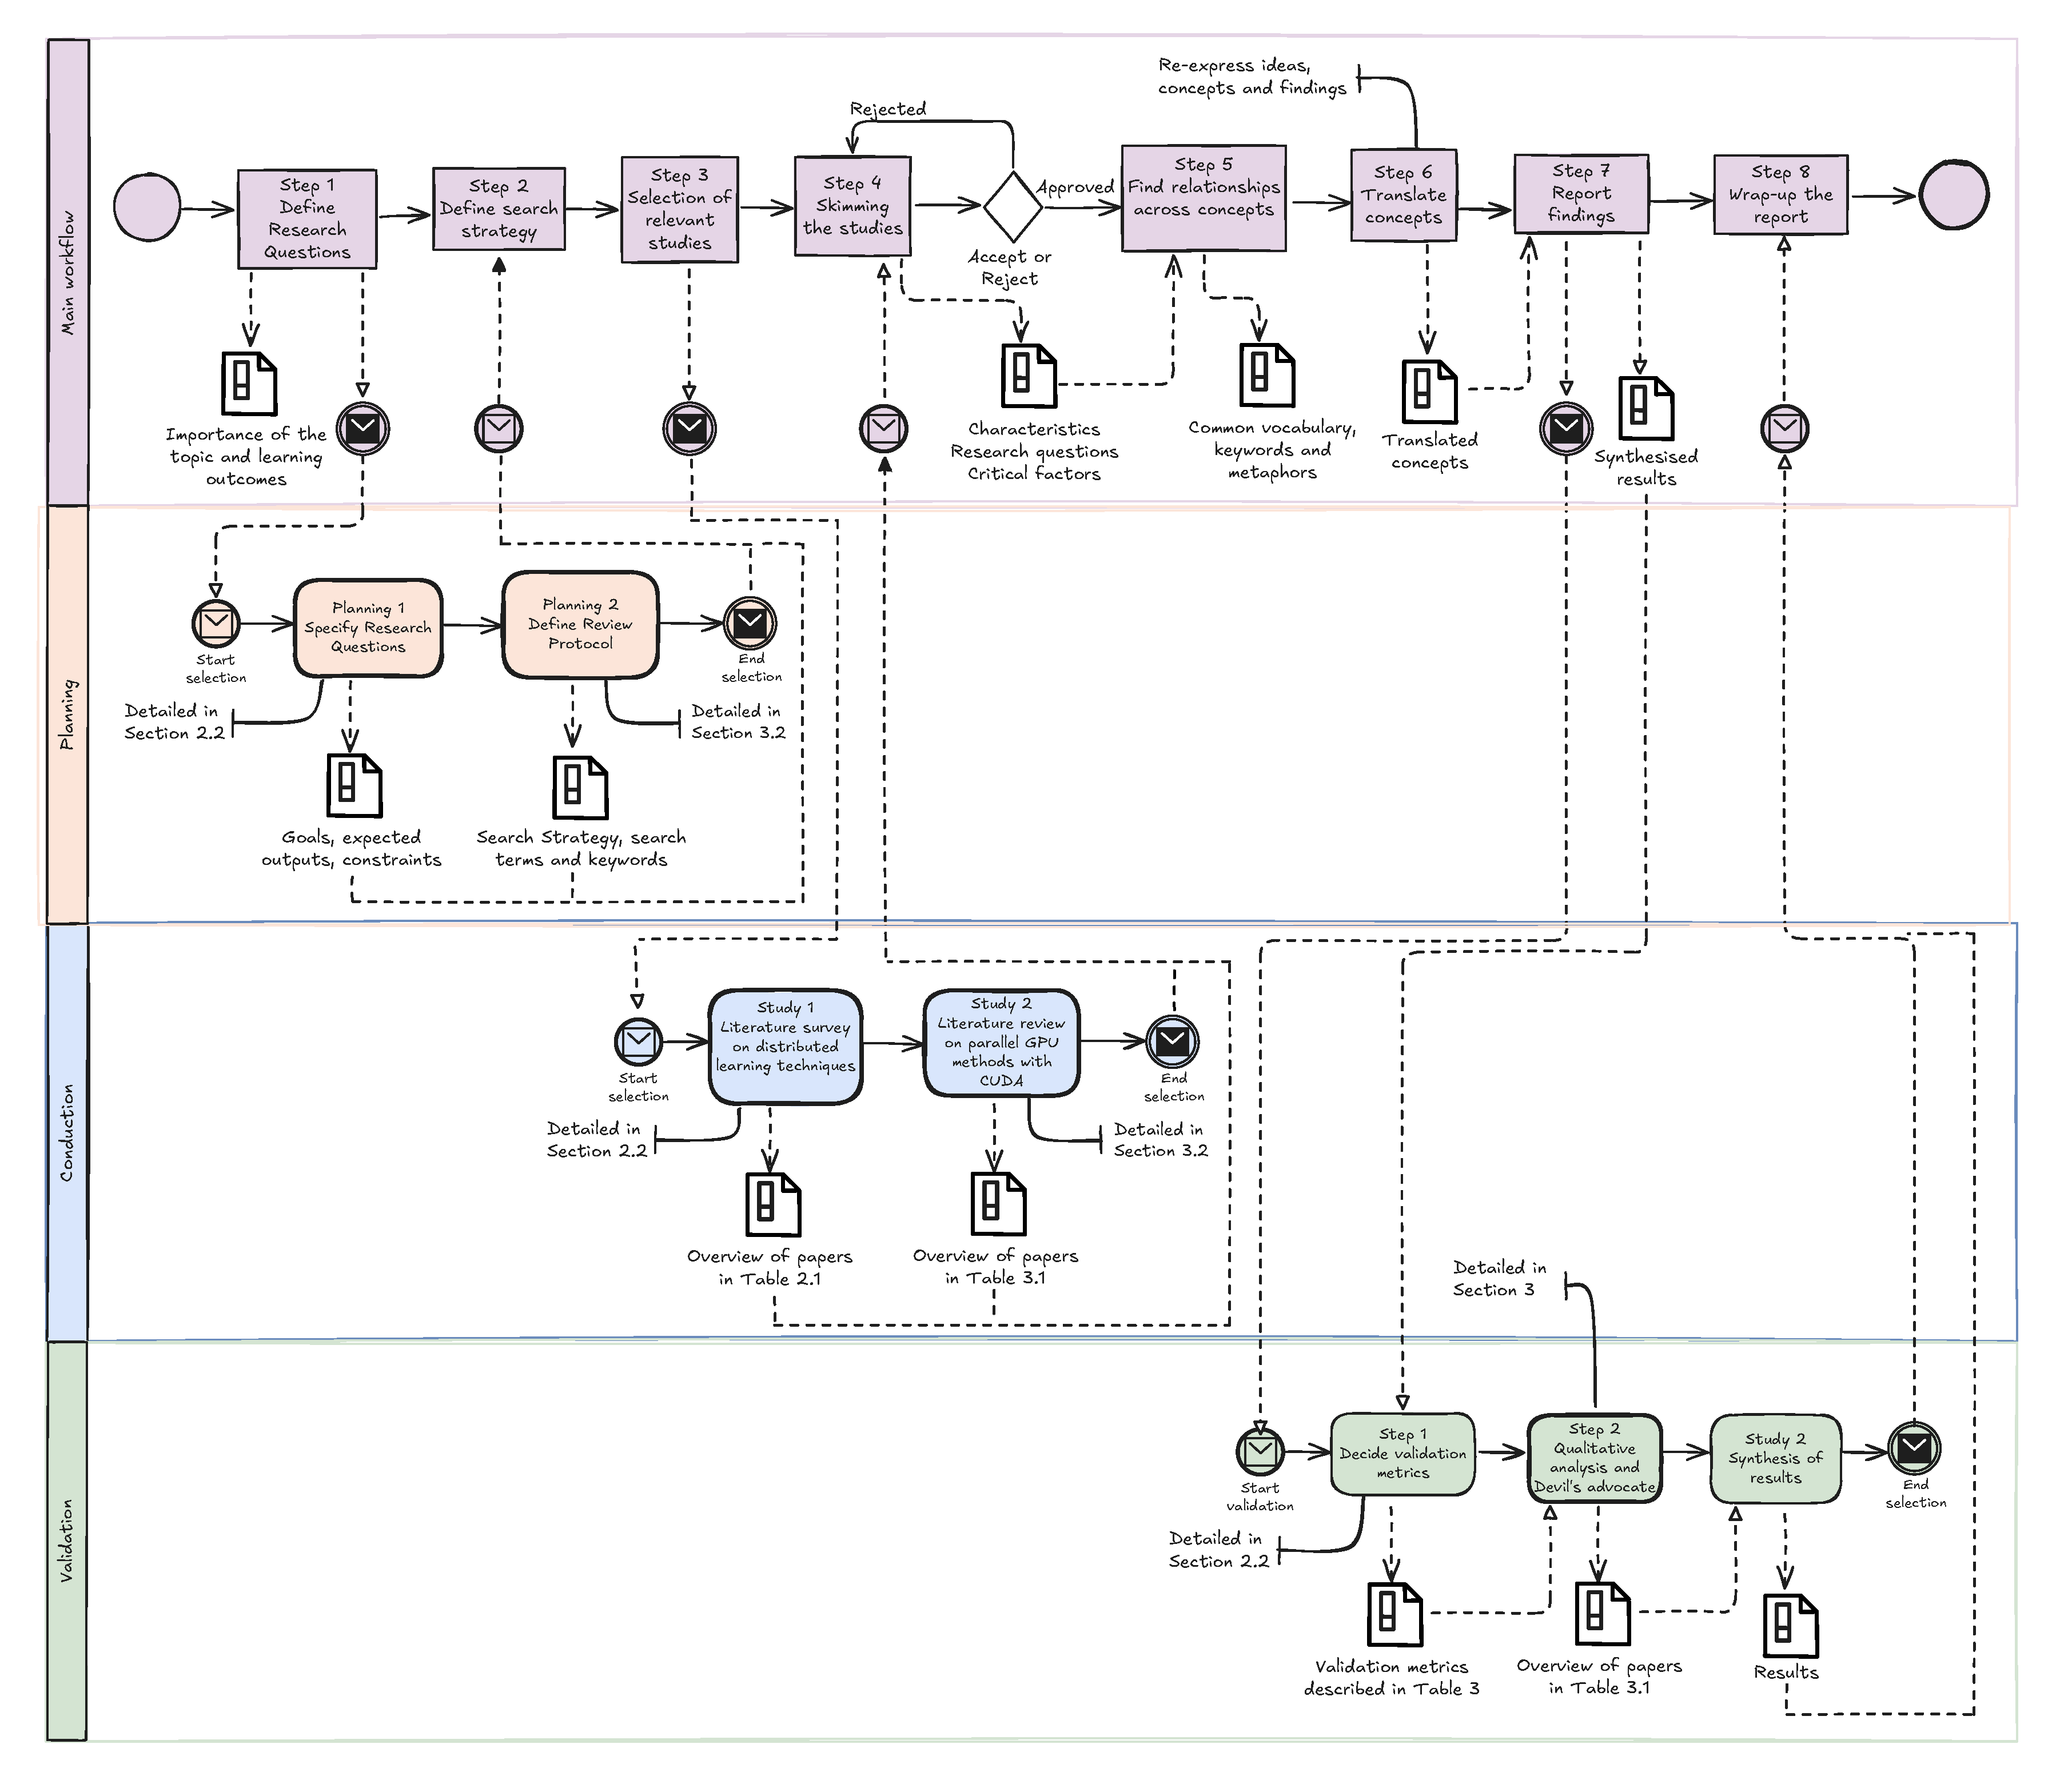
\includegraphics[width=\linewidth]{figures/workflow2}
	\caption{Systematic review workflow showing the main steps, documentation artifacts, and validation processes.
		The workflow is divided into three main phases: main workflow (top), studies selection (middle), and
		validation (bottom). Dashed lines indicate documentation and communication flows. Adapted from \cite{dos_santos_sustainable_2024}.}
	\label{fig:workflow}
\end{figure*}

\section{Related Work}
\label{sec:related_work}

\TODO{Reference the related work on survying the present methods both in DDL and CUDA}

Related work focuses on techniques and algorithms for training deep learning models across multiple
machines \cite{dehghani_distributed_2023, chahal_hitchhikers_2018, berloco_systematic_2022}. These
sources explore various aspects of DDL, such as parallelization techniques and communication
methods. However, our contribution emphasizes the connection between DDL and GPU programming with
CUDA. Furthermore, this study details the main libraries for DDL and GPU programming. We will also
provide practical guidance on running a small neural network in CUDA and facilitating PyTorch
Distributed Data Parallel (DDP) programming using Docker, addressing a practical implementation gap
not covered in the previous work. \TODO{Highlight related surveys concerning CUDA}

This study follows primarily the guidelines described in \cite{keele_systematic_2007}, however
advice for conducting the review is synthesized from a wider range of related articles
\cite{brereton_lessons_2007-1,kitchenham_procedures_nodate,budgen_reporting_2018,dos_santos_sustainable_2024}.

Distributed training of neural networks has become essential for modern deep learning applications
due to increasing model complexity and dataset sizes \cite{chahal_hitchhikers_2018}. The main
approaches for distributing neural network training can be categorized into several key strategies
\cite{dehghani_distributed_2023}:

\begin{itemize}
	\item \textbf{Data Parallelism:}
	      The dataset is divided across multiple nodes, with each node training a complete copy of the
	      model on its portion of data. Gradients from all nodes are then combined to update the model parameters.
	      This approach can be implemented either synchronously (all nodes wait for each other) or asynchronously (nodes work independently).

	\item \textbf{Model Parallelism:}
	      The neural network model itself is divided across different nodes, with each node responsible
	      for computing a specific portion of the model architecture. This strategy is particularly useful
	      when the model is too large to fit on a single machine.

	\item \textbf{Pipeline Parallelism:}
	      The training process is divided into sequential stages, similar to an assembly line,
	      where the output of one stage becomes the input for the next. This allows different parts
	      of the model to train simultaneously while maintaining dependencies.

	\item \textbf{Hybrid Parallelism:}
	      This approach combines multiple parallelization strategies to optimize training efficiency.
	      For example, model parallelism might be used to distribute a large model across GPUs, while
	      data parallelism is applied to each model segment.
\end{itemize}

These approaches can be further enhanced through techniques such as gradient compression, mixed
precision training, and tensor fusion \cite{dehghani_distributed_2023}. The choice of specific
techniques depends on factors including model architecture, available hardware, and training
requirements. For a comprehensive review of these techniques and their implementations, readers are
referred to \cite{chahal_hitchhikers_2018}.

\section{Research method}
\label{sec:protocol}

Multiple studies in the literature emphasize that a literature survey should be both transparent
and replicable \cite{keele_systematic_2007, dos_santos_sustainable_2024-1}, the main reason being
that this allows to minimize reviewer bias. This is a valid concern in general, however especially
so in this survey since it is conducted by only one person. In a broader study, bias would normally
be minimized by having multiple iterations with more than one reviewer involved. In this paper,
steps have been taken to mitigate this bias, acknowledging that it is not possible to eliminate it
completely. To ensure this, the process is documented and most of the resulting artifacts are
present in the text and in the Appendix. Moreover, AI classifiers were used during the screening
process to make the selection manageable by one person. The details are provided in Section
\ref{sec:ai-screening}.

% TODO these are all good but was hoping to minimize the number of citations
% TODO \cite{keele_systematic_2007,brereton_lessons_2007-1,budgen_reporting_2018, dos_santos_sustainable_2024-1},

% Now detail Step 1 content
The workflow is shown in Figure \ref{fig:workflow} where the key phases are annotated as follows:
Getting Started (M.1, M.2), Planning the Review (M.3, M.4), Conducting the Review (M.5, M.6), and
Reporting the Review (M.7, M.8). M.2 calls an auxiliary process composed of S.1 and S.2 to select
the appropriate studies \TODO{add references across the paper}.

\subsection{M.1 -- The need for a survey}
\label{sec:need_for_survey}

\textbf{Importance of the topic.}
Distributed techniques are important in neural networks because they allow models with billions of
parameters to perform a large number of computations in a reasonable amount of time. One of the
pioneering papers in machine learning that made use of GPUs to train neural networks in parallel
(AlexNet \cite{krizhevsky_imagenet_2012}), mentioned that the network took "between five and six days to
train on two GTX 580 3GB GPUs", suggesting that the training time would have taken much longer on a
CPU.

One key property of distributing neural network architectures to a larger number of parameters, is
that one can achieve better generalization and lower error rates even when training on smaller
datasets \cite{kaplan_scaling_2020}. This gives the impression of intelligence due to the model's
ability to make predictions that seem insightful. Understanding innate details on how these
libraries function, can provides a fertile foundation for future ideas.

\textbf{Learning outcomes.}
As a result of conducting the survey I expect the following learning outcomes: learn from the primary
studies, improve writing and research skills, gain practical experimental expertise using CUDA and
Pytorch DDP and identify potential research ideas for future projects.

\subsection{M.2 -- Getting started}
\label{sec:research_questions}
Building on the learning outcomes defined in Section \ref{sec:need_for_survey}, we define
the goals, expected outputs and constraints. The main goal was to analyze parallelization frameworks in DDL and CUDA.
The expected results were to identify key frameworks for each category. For this, we defined two main constraints: (i)
we only considered frameworks that introduce CUDA and DDL frameworks and (ii) we included only primary
studies that were peer-reviewed, although literature surveys were used to gain familiarity with the topic,
however they are only discussed in Section \ref{sec:related_work}. These ideas are formally defined
in Section \TODO{...} and \TODO{...}.

\subsection{M.3 -- Selection of Relevant Studies}
This step identified and selected studies from both areas (CUDA programming and DDL). I collected
studies of the state of the art of both CUDA frameworks (in Step S.1) and DDL libraries (in Step
S.2).

\subsubsection{S.1 -- Survey on CUDA programming libraries}
\paragraph{S.1.1 -- Problem definition.}
In order to identify interesting frameworks and broaden the understanding of the topic, I conducted
a secondary study\footnote{A secondary study synthesizes primary papers to provide a comprehensive
	overview. This contrasts with tertiary studies which analyze secondary studies.}. This decision was
made in the problem definition step (S.1.1 in Figure \ref{fig:workflow-study}). In order to do this
systematically, this section defines a research protocol during the planning phase, which is then
used to find related studies. The research protocol is essentially a framework for conducting the
review. This section outlines the key decisions that were made with to create the protocol by
identifying the research questions and search strategy.

\begin{figure*}[th]
	\centering
	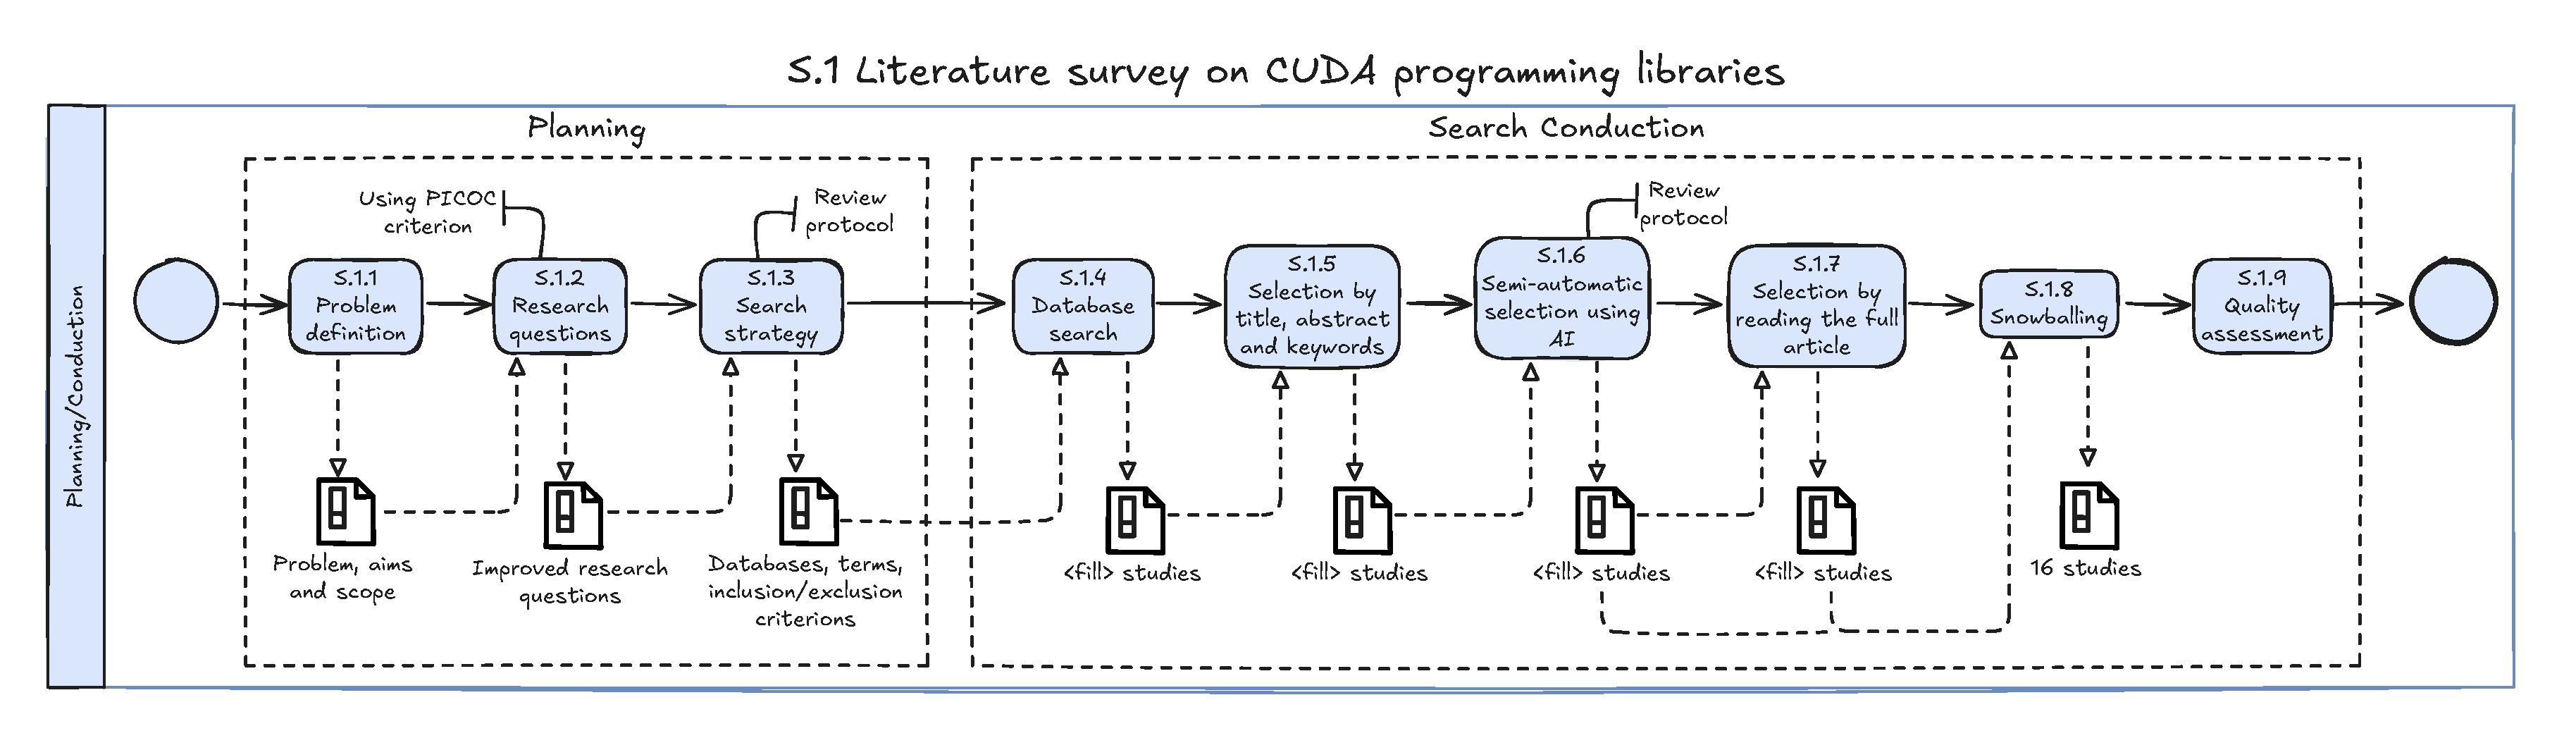
\includegraphics[width=\linewidth]{figures/workflow3}
	\caption{The diagram suggests the key steps for finding papers related to the CUDA programming survey. The phases
		include planning the review (aims, research questions, search strategy) and conducting the review (study selection phase). The research questions
		were transformed according to the PICOC (Population, Intervention, Comparison, Outcome, Context) criterion suggested by \cite{keele_systematic_2007}.}.
	\label{fig:workflow-study}
\end{figure*}

\paragraph{S.1.2 -- Research questions.}
After an initial literature review, the research questions (RQ) defined in Section
\ref{sec:initial_research_questions} are refined using the guidelines defined in
\cite{kitchenham_evidence-based_2015} and \cite{keele_systematic_2007}. Specifically, the PICOC
(Population, Intervention, Comparison, Outcome, Context) criterion is used to transform the
questions into a format that ensures them to be specific, measurable and well-defined. The
questions below are ordered based on their significance in the survey:

% TODO: remove this
% \begin{itemize}
% 	\item \textbf{RQ\textsubscript{1}} What are the most common frameworks currently available for 
% 		  GPU programming with CUDA, and how do their usability compare?
% 		  % NOTE implementing distributed deep learning, and how does their usability compare?
% 	      % NOTE \cite{berloco_systematic_2022, ben-nun_demystifying_2020, langer_distributed_2020}?
% 	      % NOTE \item How do parameter update strategies impact distributed deep learning systems (e.g., Parameter Server and decentralised approaches) \cite{ben-nun_demystifying_2020,berloco_systematic_2022,langer_distributed_2020}?
% 	\item How is stochastic gradient descent (SGD) computed in distributed environments
% 	      \cite{berloco_systematic_2022,ben-nun_demystifying_2020,langer_distributed_2020,verbraeken_survey_2021}? % NOTE and what are the associated challenges 
% 	\item What are the key frameworks currently available for implementing DDL, and how do their features 
% 	      compare \cite{berloco_systematic_2022}?
%  	\item In what ways are the techniques used in DDL also useful in GPU parallelization?
% \end{itemize}

% TODO: \TODO{RQ1: ease of learning, ease of use and documentation compare?}

\begin{itemize}
	\item \textbf{RQ\textsubscript{1}:} In the field of Deep Learning, what are the most frequently cited
	      frameworks for GPU programming using CUDA, and how do their user communities differ in size? \\
	      \textit{Rationale:} By identifying the most common frameworks, we can identify which are the gaps
	      in the literature they cover and which are the most promising areas for future research.

	\item \textbf{RQ\textsubscript{2}:} In the field of Deep Learning, what are the most commonly cited
	      frameworks for distributed training of neural networks across clusters, and how do their respective user communities vary in size? \\
	      \textit{Rationale:} By identifying the most common frameworks, we can trace the years in which they were published
	      and form a unified timeline of the evolution of the field with respect to the related CUDA programming advancements.

	      % NOTE Razvan I am conducting a literature review in the field of deep learning, specifically focusing on distributed training of 
	      % NOTE neural networks across clusters. I need to identify the most commonly cited frameworks used for this purpose.
	\item \textbf{RQ\textsubscript{3}:} What practical applications of these technologies have been reported in the literature? \\
	      \textit{Rationale:} This can yield hands-on experience on the topic which is helpful for practical applications.
	\item \textbf{RQ\textsubscript{4}:} What are the overlaps in data/model optimization strategies used in DDL and GPU parallelization? \\
	      \textit{Rationale:} By identifying the overlaps, it offers a more unified view of how the concepts are interrelated.
\end{itemize}

The questions play a key role in guiding the search strategy, data extraction process and results
synthesis phase.

\paragraph{S.1.3 -- Search Strategy.}
The search strategy represents represents a systematic approach for identifying relevant studies
that adequately answer the research questions.

\paragraph{Databases.}
The process involves a manual search of four citation databases --
\href{https://ieeexplore.ieee.org/}{IEEE Xplore}, \href{https://dl.acm.org/}{ACM Digital Library},
\href{https://www.sciencedirect.com/}{Science Direct}, and \href{https://www.scopus.com/}{Scopus}
-- that include conference proceedings and journal papers, considering three metadata fields
(title, abstract, and keywords).

\paragraph{Inclusion/Exclusion Criteria.}
There were defined four inclusion criteria (IC) and three exclusion criteria (EC). In particular, I
decided to select only primary studies, however secondary studies were mentioned in Section
\ref{sec:related_work}. The identification of secondary studies was useful since the selected
studies synthesize evidence and can make it possible to access primary studies:

\begin{itemize}
	\item \textbf{IC\textsubscript{1}}: Study is a primary study and is peer-reviewed.
	\item \textbf{IC\textsubscript{2}}: Study addresses distributed frameworks in DL.
	\item \textbf{IC\textsubscript{3}}: Study addresses GPU programming with CUDA.
	\item \textbf{IC\textsubscript{4}}: Study introduces a library or a framework. \\
	\item \textbf{EC\textsubscript{1}}: Study does not discuss implementation details.
	\item \textbf{EC\textsubscript{2}}: Study is not a primary study.
	\item \textbf{EC\textsubscript{3}}: Study is not written in English.
\end{itemize}

\paragraph{Search terms.}
In Step S.1.3, I inquired about the literature using the following search string:
\begin{quote}
	\textit{( "machine learning" OR "deep learning" )
		AND
		( "Data parallelism" OR "model parallelism")
		AND
		( "framework" OR "implementation" )}
\end{quote}

While in Step S.2.3, the following search string was used \TODO{review string}:
\begin{quote}
	\textit{( "machine learning" OR "deep learning" )
		AND
		( "Data parallelism" OR "model parallelism")
		AND
		( "framework" OR "implementation" )}
\end{quote}

The details and justification to define this search string can be found in the supplementary
material in Section \ref{sec:search_strategy}.

\paragraph{Publication year criteria.}
The search was restricted to papers published between $\yearstartcuda$-$\yearendcuda$ for the CUDA
task and $\yearstartddl$-$\yearendddl$ for the DDL task. The former start year ($\yearstartcuda$)
was chosen as the baseline due to being the year when AlexNet \cite{krizhevsky_imagenet_2012} was
published. This paper revolutionized research in neural networks by allowing advanced AI models to
be trained on GPUs.

The latter start year ($\yearstartddl$) was chosen as at this point there was a shift towards
resource conservation, which resulted in a focus on concurrency within mini-batches
\cite{ben-nun_demystifying_2020}. This is the year by which the effectiveness of deep learning
algorithms was more widely recognized and more research was published that focused on scalability.

\paragraph{S1.4 - S1.5 -- Study selection}
After an initial database search (Step S1.4), \todo{fill-me} studies were retrieved. A selection
process was initiated by reading the title, abstract and keywords of each study (S.1.5), resulting
in \todo{fill-me} studies.

\paragraph{S1.6. -- Semi-automatic selection using AI}
\label{sec:ai-screening}
Next, as suggested in \cite{brereton_lessons_2007-1}, I applied
AI inference engines to filter resulting studies into a more easily digestible set (S.1.6). The technique
is semi-automatic with a focus on screening and extraction of relevant information.

\begin{table}[htbp]
	\centering
	\caption{The Search Engines Used in this Survey}
	\label{tab:databases}
	\begin{tabular}{llllr}
		\hline
		ID & Tool           & Stage  & Mode    & Number of uses \\
		\hline
		1  & IEEExplore     & Search & Web     & 33             \\
		2  & ACM            & Search & Web     & 30             \\
		3  & ScienceDirect  & Search & Web     & 24             \\
		4  & Web of Science & Search & Web     & 19             \\
		5  & Google Scholar & Search & Web     & 18             \\
		6  & SpringerLink   & Search & Web     & 17             \\
		7  & Scopus         & Search & Web     & 14             \\
		8  & Compendex      & Search & Desktop & 11             \\
		9  & CiteSeer       & Search & Web     & 5              \\
		\hline
	\end{tabular}
\end{table}

\begin{table}[htbp]
	\centering
	\caption{\footnotesize Number of studies before and after applying the IC and EC}
	\label{tab:criteria}
	\begin{tabular}{lrrrrr}
		\hline
		                           & \footnotesize IEEE   & \footnotesize Science & \footnotesize Scopus & \footnotesize ACM     & \footnotesize Total \\
		                           & \footnotesize Xplore & \footnotesize Direct  &                      & \footnotesize Library &                     \\
		\hline
		\footnotesize Before IC/EC & 22                   & 10                    & 10                   & 30                    & 72                  \\
		\footnotesize After IC/EC  & 10                   & 10                    & 10                   & 30                    & 60                  \\
		\hline
	\end{tabular}
\end{table}

% ===== STEP 3: Selection of Relevant Studies =====
% This section details:
% - Study 1: Distributed learning techniques
% - Study 2: CUDA implementations

% Combined "Purpose," "Scope," and "Relationship Between Study Types"
This section defines the aims and scope of the review, clarifying the types of studies to be
included and the rationale for exploring distributed learning and CUDA implementations together.
The specific objectives of the review are aligned with the associated research questions to provide
a clear focus. The boundaries of the review concern the types of distributed learning techniques
and CUDA implementations considered, with a time period between 2015 and 2022 to ensure currency.
The review includes studies focusing on the design and analysis of distributed learning algorithms
and those focusing on CUDA-based parallel implementations to understand the translation of
theoretical aspects into practical implementations. This approach allows for the exploration of
patterns and challenges in mapping distributed algorithms onto parallel architectures
\TODO{Different topics explored together}.

\subsubsection{Distributed Learning Techniques Review}
The review will focus on distributed learning approaches, aligning with "Study 1" in Figure
\ref{fig:workflow}, with the following considerations:
\begin{itemize}
	\item Types of algorithms including \textbf{data parallelism, model parallelism, and asynchronous
		      Stochastic Gradient Descent (SGD)} \cite{ben-nun_demystifying_2020,langer_distributed_2020}.
	\item Different distributed architectures including parameter servers and peer-to-peer systems
	      \cite{verbraeken_survey_2021,ben-nun_demystifying_2020,langer_distributed_2020}.
	\item Specific machine learning models such as neural networks and support vector machines.
\end{itemize}

\subsubsection{CUDA-based Parallel Implementation Review}
For CUDA implementations, the review will consider aspects relevant to "Study 2" in Figure
\ref{fig:workflow}:
\begin{itemize}
	\item Implementation of distributed methods on NVIDIA GPUs using the CUDA framework
	\item Different CUDA libraries and architectures
	\item Specific hardware considerations including GPUs and Tensor Processing Units (TPUs)
\end{itemize}

\subsubsection{Justification for Inclusion}
Both distributed learning techniques and CUDA implementation studies will be included to provide a
complete picture of the current state-of-the-art research in the area. By including both study
types, a deeper understanding of both theoretical approaches and implementation techniques for
practical applications can be reached.

\subsection{Preliminary Protocol Development}
This systematic review follows the guidelines proposed by Kitchenham and Charters for software
engineering research. The preliminary review protocol was developed to establish the foundation for
the steps visualized in Figure \ref{fig:workflow}, particularly in the initial stages. An overview
of the papers included after the initial selection phase (corresponding to the output of the
"Studies Selection" phase in Figure \ref{fig:workflow}) will be presented in Table 2.1.

\subsubsection{Background and Rationale}
This section provides the necessary context for the review, outlining the research gaps that will
be addressed \cite{ben-nun_demystifying_2020}. It explicitly states the need for a systematic
review of the current literature to address this gap and provide a focused analysis.

\subsubsection{Initial Search Strategy}
The initial search strategy involves combining keywords using Boolean and proximity operators to
generate search strings, based on the "Goals, expected outputs, constraints, search terms and
keywords" documented as an input to Step 1 in Figure \ref{fig:workflow}. Databases like Scopus,
Google Scholar, and ACM Digital Library are selected for their coverage of computer science,
engineering, and applied mathematics literature. Studies published between 2015-2022 will be
considered to ensure recent advancements are included while maintaining a consistent period for
analysis.
\begin{itemize}
	\item \textbf{Search Terms:} Details of the search terms will be provided in Section \ref{sec:search_process_documentation}.
	\item \textbf{Database Justification:} Rationale for selecting specific databases is detailed in Section \ref{sec:search_process_documentation}.
	\item \textbf{Timeline:} The timeframe for including studies is 2015-2022.
\end{itemize}

\subsubsection{Preliminary Selection Criteria}
Preliminary criteria for inclusion will use specific examples such as ``studies that evaluate the
performance of synchronous distributed SGD in deep learning models'' rather than general terms like
``distributed computing'' \cite{ben-nun_demystifying_2020}. Preliminary quality thresholds will
ensure only high-quality studies are included in the final analysis. Specific inclusion and
exclusion criteria are detailed in Section \ref{sec:study-selection-criteria}.

\subsubsection{Initial Data Extraction Plan}
The following information will be extracted from each study:
\begin{itemize}
	\item Details of distributed systems \cite{ben-nun_demystifying_2020,langer_distributed_2020}:
	      \begin{enumerate}
		      \item Number of nodes
		      \item Communication network
		      \item Communication method
		      \item Topology
	      \end{enumerate}
	\item Machine learning algorithms and models used \cite{xing_strategies_2015}.
	\item Datasets and benchmarks \cite{ben-nun_demystifying_2020}.
	\item Performance metrics (training time, accuracy, speedup)
	      \cite{ben-nun_demystifying_2020,langer_distributed_2020,xing_strategies_2015}.
	\item CUDA implementation details (libraries, optimizations)
	      \cite{verbraeken_survey_2021,ben-nun_demystifying_2020,xing_strategies_2015}.
\end{itemize}
Further details on the data extraction strategy can be found in Section \ref{sec:data-extraction-strategy}.

\subsubsection{Quality Assessment Framework}
Preliminary quality assessment will use specific criteria to evaluate the validity and reliability
of methods, using established checklists from the literature \cite{ben-nun_demystifying_2020}. A
Likert scale will be used for a standardized approach. Detailed guidelines for reviewers will be
established to ensure consistency and prevent bias, as described further in Section
\ref{sec:quality-assessment-process}.
\begin{itemize}
	\item \textbf{Criteria:} Specific criteria are detailed in Section \ref{sec:quality-assessment-process}.
	\item \textbf{Scoring System:} A Likert scale will be used.
	\item \textbf{Guidelines:} Guidelines for reviewers are detailed in Section \ref{sec:quality-assessment-process}.
\end{itemize}

\subsubsection{Synthesis Approach}
The synthesis approach will involve meta-analysis where appropriate, using statistical analysis to
combine results from included studies with clearly defined methods
\cite{ben-nun_demystifying_2020}. Thematic synthesis will be used for narrative synthesis, allowing
an in-depth understanding of themes present in selected studies.
\begin{itemize}
	\item \textbf{Meta-analysis:} Details of the methods will be defined later.
	\item \textbf{Narrative synthesis:} Thematic synthesis will be employed.
\end{itemize}

\subsection{Search Process Documentation}
\label{sec:search_process_documentation}
This section provides an overview of our search strategy. Detailed search documentation, including exact search strings and results for each database, can be found in the supplementary materials (Section \ref{sec:search_strategy}).

\subsubsection{Search Strategy Overview}
Our search strategy combines terms from two main categories as shown in Table
\ref{tab:search_terms}. The number of articles retrieved from each database is presented in Table
\ref{tab:search_results}.

\begin{table*}[ht]
	\centering
	\caption{Number of Retrieved Articles by Database}
	\label{tab:search_results}
	\begin{tabular}{|l|c|c|c|}
		\hline
		\textbf{Database}   & \textbf{Initial Results} & \textbf{After Filtering} & \textbf{Final Selection} \\
		\hline
		Scopus              & XXX                      & XXX                      & XXX                      \\
		\hline
		Google Scholar      & XXX                      & XXX                      & XXX                      \\
		\hline
		ACM Digital Library & XXX                      & XXX                      & XXX                      \\
		\hline
		IEEE Xplore         & XXX                      & XXX                      & XXX                      \\
		\hline
		Science Direct      & XXX                      & XXX                      & XXX                      \\
		\hline
		arXiv               & XXX                      & XXX                      & XXX                      \\
		\hline
		\textbf{Total}      & XXX                      & XXX                      & XXX                      \\
		\hline
	\end{tabular}
\end{table*}

The complete search strings for each database, including any database-specific adaptations, are
documented in Section \ref{sec:search_strategy} of the supplementary materials.

\subsection{Study Selection Criteria}
\label{sec:study-selection-criteria}
This section specifies the detailed inclusion and exclusion criteria for the studies to be included
in the review. These will be specific, measurable, and objective to ensure that all studies are
assessed consistently and fairly \cite{ben-nun_demystifying_2020}.

% TODO: Razvan. Is this fine?
\subsubsection{Inclusion Criteria}
The following criteria will be used for including studies:
\begin{itemize}
	\item Studies published between 2013 and 2023
	\item Peer-reviewed articles and high-quality preprints
	\item Studies focusing on distributed training techniques
	\item Articles written in English
	\item Implementation details available
\end{itemize}
\cite{verbraeken_survey_2021,ben-nun_demystifying_2020}.

\subsubsection{Exclusion Criteria}
Studies will be excluded based on the following criteria:
\begin{itemize}
	\item Studies not focused on neural network training
	\item Pure theoretical papers without implementation
	\item Secondary studies (surveys, reviews)
	\item Insufficient technical details or results
\end{itemize}

\subsection{Quality Assessment Process}
\label{sec:quality-assessment-process}
This part of the methodology details the process used to assess the quality of the selected studies, aligning with the "Validation" phase shown in the bottom section of Figure \ref{fig:workflow}.

\subsubsection{Quality Criteria}
The quality of the studies will be evaluated based on the methodological rigour, clarity of
reporting, limitations of the studies, and potential for bias. Established checklists, such as
those provided by the CASP, will be used to address bias and validity in a rigorous and systematic
way.

\subsection{Data Extraction Strategy}
\label{sec:data-extraction-strategy}
This section details how data will be extracted from the included studies. The data extraction form will be designed to capture all necessary information, including study details, methodology, implementation specifics, dataset details, and results. The form will be piloted to ensure it captures the information effectively \cite{ben-nun_demystifying_2020}.

% \subsubsection{Extraction Form}
% The data extraction form was iteratively refined through:

% TODO Razvan
% \begin{itemize}
%     \item Publication metadata
%     \begin{itemize}
%         \item Authors, venue, year
%         \item Citation count and impact
%     \end{itemize}
%     \item Technical details
%     \begin{itemize}
%         \item Distributed training approach
%         \item Implementation specifications
%         \item Hardware configurations
%     \end{itemize}
%     \item Performance metrics
%     \begin{itemize}
%         \item Training time and convergence
%         \item Resource utilization
%         \item Scalability measures
%     \end{itemize}
%     \item Experimental setup
%     \begin{itemize}
%         \item Dataset characteristics
%         \item Hardware specifications
%         \item Software frameworks used
%     \end{itemize}
% \end{itemize}

\begin{itemize}
	\item \textbf{Details:} The data extraction form will capture study design, participants, interventions, and outcomes, as well as details of the implementation in distributed systems and parallel CUDA frameworks \cite{ben-nun_demystifying_2020}.
	\item \textbf{Piloting:} The extraction form will be piloted to ensure effectiveness \cite{ben-nun_demystifying_2020}.
	\item \textbf{Study Details:} The form will capture relevant details including implementation specifics.
\end{itemize}

% Final paragraph about methodology
By using this methodology, the systematic review will aim to provide a comprehensive and reliable
analysis of the current state of research in distributed deep learning and CUDA implementations.
The approach used here will enable the review to identify any trends and gaps in current research
and make recommendations for future study.

\subsection{Study Selection Results}
\label{sec:study_selection_results}
The complete lists of included and excluded studies, along with detailed information about each study, can be found in the supplementary materials (Section \ref{sec:study_selection}). A total of XXX studies were initially identified, with XXX studies meeting our inclusion criteria after screening. Table \ref{tab:study_types} provides an overview of the types of studies included in our review.

\begin{table*}[ht]
	\centering
	\caption{Overview of Included Study Types}
	\label{tab:study_types}
	\begin{tabular}{|l|c|p{8cm}|}
		\hline
		\textbf{Study Type}    & \textbf{Count} & \textbf{Description}                                                     \\
		\hline
		Empirical Studies      & XXX            & Studies with experimental evaluations of distributed learning techniques \\
		\hline
		Implementation Studies & XXX            & Studies focusing on CUDA implementations and optimizations               \\
		\hline
		Hybrid Studies         & XXX            & Studies covering both theoretical and implementation aspects             \\
		\hline
		\textbf{Total}         & XXX            &                                                                          \\
		\hline
	\end{tabular}
\end{table*}

\begin{itemize}
	\item \textbf{Goals:}
	\item To analyze parallelization frameworks in DDL.
	\item To evaluate libraries that support CUDA programming.
	\item To find out how these concepts are intertwined.
	\item To get practical experience with popular frameworks. \\
	\item \textbf{Expected Outputs:}
	\item Experience for conducting a systematic review.
	\item Systematic mapping of programming frameworks.
	\item Comparative analysis with strengths and weaknesses.
	\item Identification of research gaps. \\
	\item \textbf{Constraints:}
	\item Time period limited to 2012-2024\footnote{CUDA: 2012 is the year when AlexNet was published.} and
	      2015-2024\footnote{DDL: 2015 is the year when the shift towards scalability was noticed.}.
	\item Peer-reviewed articles and conference papers only.
	\item English language publications only.
	\item Technical implementation details must be present. \\
	\item \textbf{Search Terms and Keywords:}
	\item Listed in Table \ref{tab:search_terms}.
\end{itemize}

\begin{table*}[htbp]
	\centering
	\caption{The DNN papers included in the review. 1 (data), 2 (model), 3 (pipeline)}
	\label{tab:dnn_papers}
	\begin{tabular}{llp{8.01cm}p{2cm}lll}
		\hline
		\textbf{\#} & \textbf{Ref.}                    & \textbf{Title}                                                                                            & \textbf{Type}  & \textbf{Year} & \textbf{Citations} & \textbf{Stars}                                                \\[1ex]
		\hline
		1           & \cite{li_pytorch_2020}           & PyTorch Distributed: Experiences on Accelerating Data Parallel Training                                   & Hybrid (1,2,3) & 2020          & 175                & 86.1k \cite{noauthor_pytorchpytorch_nodate}                   \\[1ex]
		2           & \cite{abadi_tensorflow_2016}     & TensorFlow: Large-Scale Machine Learning on Heterogeneous Distributed Systems                             & Data           & 2016          & 9998               & 187k \cite{abadi_tensorflow_2015}                             \\[1ex]
		3           & \cite{wolf_huggingfaces_2020}    & HuggingFace's Transformers: State-of-the-art Natural Language Processing                                  & Data           & 2020          & 1444               & 8.2k \cite{noauthor_huggingfaceaccelerate_2025}               \\[1ex]
		4           & \cite{noauthor_overview_nodate}  & The lightweight PyTorch wrapper for high-performance AI research. Scale your models, not the boilerplate. & Data           & 2019          & N/A                & 28.8k \cite{falcon_pytorch_2019}                              \\[1ex]
		5           & \cite{frostig_compiling_nodate}  & Compiling machine learning programs via high-level tracing                                                & Hybrid         & 2018          & 297                & 31k \cite{noauthor_jax-mljax_2025}                            \\[1ex]
		6           & \cite{shoeybi_megatron-lm_2020}  & Megatron-LM: Training Multi-Billion Parameter Models for Natural Language Processing                      & Hybrid         & 2020          & 1578               & 11.2k \cite{noauthor_nvidiamegatron-lm_2025}                  \\[1ex]
		7           & \cite{huang_gpipe_2019}          & GPipe: Efficient Training of Giant Neural Networks using Pipeline Parallelism                             & Pipeline       & 2018          & 1446               & 2.8k \cite{noauthor_tensorflowlingvo_2025}                    \\[1ex]
		8           & \cite{rasley_deepspeed_2020}     & DeepSpeed: System Optimizations Enable Training Deep Learning Models with Over 100 Billion Parameters     & Hybrid         & 2020          & 1059               & 36.3k \cite{noauthor_microsoftdeepspeed_2025}                 \\[1ex]
		9           & \cite{noauthor_fairscale_nodate} & FairScale:  A general purpose modular PyTorch library for high performance and large scale training       & Hybrid         & 2021          & N/A                & 3.2k \cite{FairScale2021}                                     \\[1ex]
		10          & \cite{noauthor_amazon_nodate}    & Amazon SageMaker Platform                                                                                 & Data           & 2017          & N/A                & 10.3k \cite{noauthor_awsamazon-sagemaker-examples_2025}       \\[1ex]
		11          & \cite{jiang_unified_nodate}      & A Unified Architecture for Accelerating Distributed DNN Training in Heterogeneous GPU/CPU Clusters        & Data           & 2020          & 338                & 3.7k \cite{noauthor_bytedancebyteps_2025}                     \\[1ex]
		12          & \cite{sdgilley_azure_nodate}     & Microsoft AzureML Platform                                                                                & Data           & 2021          & N/A                & 1.8k \cite{noauthor_azureazureml-examples_2025}               \\[1ex]
		13          & \cite{noauthor_vertex_nodate}    & Google Vertex AI Platform                                                                                 & Data           & 2021          & N/A                & 178 \cite{noauthor_googlecloudplatformvertex-ai-samples_2025} \\[1ex]
		14          & \cite{lepikhin_gshard_2020}      & GShard: Scaling Giant Models with Conditional Computation and Automatic Sharding                          & Model          & 2020          & 931                & 2.8k \cite{noauthor_tensorflowlingvo_2025}                    \\[1ex]
		15          & \cite{li_colossal-ai_2023}       & Colossal AI: A Unified Deep Learning System for Large-Scale Parallel Training                             & Hybrid         & 2023          & 118                & 39k \cite{noauthor_hpcaitechcolossalai_2025}                  \\[1ex]
		16          & \cite{moritz_ray_2018}           & Ray: A distributed Framework for Emerging AI Applications                                                 & Hybrid         & 2018          & 1108               & 35k \cite{noauthor_ray-projectray_2025}                       \\[1ex]
		17          & \cite{sergeev_horovod_2018}      & Horovod: fast and easy distributed deep learning in TensorFlow                                            & Data           & 2018          & 1152               & 14.3k \cite{noauthor_horovodhorovod_2025}                     \\[1ex]
		\hline
	\end{tabular}
\end{table*}

% \begin{table*}[htbp]
% 	\centering
% 	\caption{The DNN papers included in the review}
% 	\label{tab2:dnn_papers}
% 	\begin{tabular}{llp{8.01cm}p{2cm}lll}
% 		\hline
% 		\textbf{\#} & \textbf{Ref.}           & \textbf{Title}                                                                & \textbf{Type} & \textbf{Year} & \textbf{Citations} & \textbf{Stars}                             \\
% 		\hline
% 		%1           & \cite{huang_gpipe_2019} & GPipe: Efficient Training of Giant Neural Networks using Pipeline Parallelism & Pipeline      & 2018          & 1446               & 2.8k \cite{noauthor_tensorflowlingvo_2025} \\
% 		2           & \cite{chen_mxnet_2015}  & MXNet: A Flexible and Efficient Machine Learning Library for Heterogeneous Distributed Systems & Hybrid (Data, Model) & 2015 & 2212 & 20.8k \cite{noauthor_apachemxnet_2025} \\
% 		% 3           & \cite{li_pytorch_2020}  & PyTorch Distributed: Experiences on Accelerating Data Parallel Training & Data & 2020 & 175 & 86.1k \cite{noauthor_pytorchpytorch_nodate} \\
% 		% 4           & \cite{abadi_tensorflow_2016} & TensorFlow: Large-Scale Machine Learning on Heterogeneous Distributed Systems & Data & 2016 & 9998 & 187k \cite{abadi_tensorflow_2015} \\
% 		% 5           & \cite{rasley_deepspeed_2020} & DeepSpeed: System Optimizations Enable Training Deep Learning Models with Over 100 Billion Parameters & Hybrid (Data, Model) & 2020 & 1059 & 36.3k \cite{noauthor_microsoftdeepspeed_2025} \\
% 		% 6           & \cite{sergeev_horovod_2018} & Horovod: fast and easy distributed deep learning in TensorFlow & Data & 2018 & 1152 & 14.3k \cite{noauthor_horovodhorovod_2025} \\
% 		% 7           & \cite{jiang_unified_nodate} & A Unified Architecture for Accelerating Distributed DNN Training in Heterogeneous GPU/CPU Clusters & Data & 2020 & 10 & 3.7k \cite{noauthor_bytedancebyteps_2025} \\
% 		% 8           & \cite{frostig_compiling_nodate} & Compiling machine learning programs via high-level tracing & Data & 2018 & 363 & 31k \cite{noauthor_jax-mljax_2025} \\
% 		\hline
% 		% Add more papers as needed
% 	\end{tabular}
% \end{table*}
